% =====================
% Chapter 8: Control Flow (Conditions and Loops)
% Audience: Architecture students new to coding
% Uses macros: \h, \hh, \hhh, \code, NoteBox, minilab
% Code tags use c08_*; each code line begins with 4 spaces at top level
% =====================

\h{Control Flow: Conditions and Loops}

Control flow is the order in which your program’s statements run. In architecture scripts,
control flow lets you \emph{branch} (choose one path) and \emph{iterate} (repeat a task)
to validate inputs, search through rooms, categorize spaces, or clean text lists.
Figure~\ref{fig:control_flow} illustrates these ideas.

\begin{figure}[h]
  \centering
  % TODO: replace the path below with the actual filename you provided
  % e.g., \includegraphics[width=\linewidth]{figs/control_flow_diagram}
  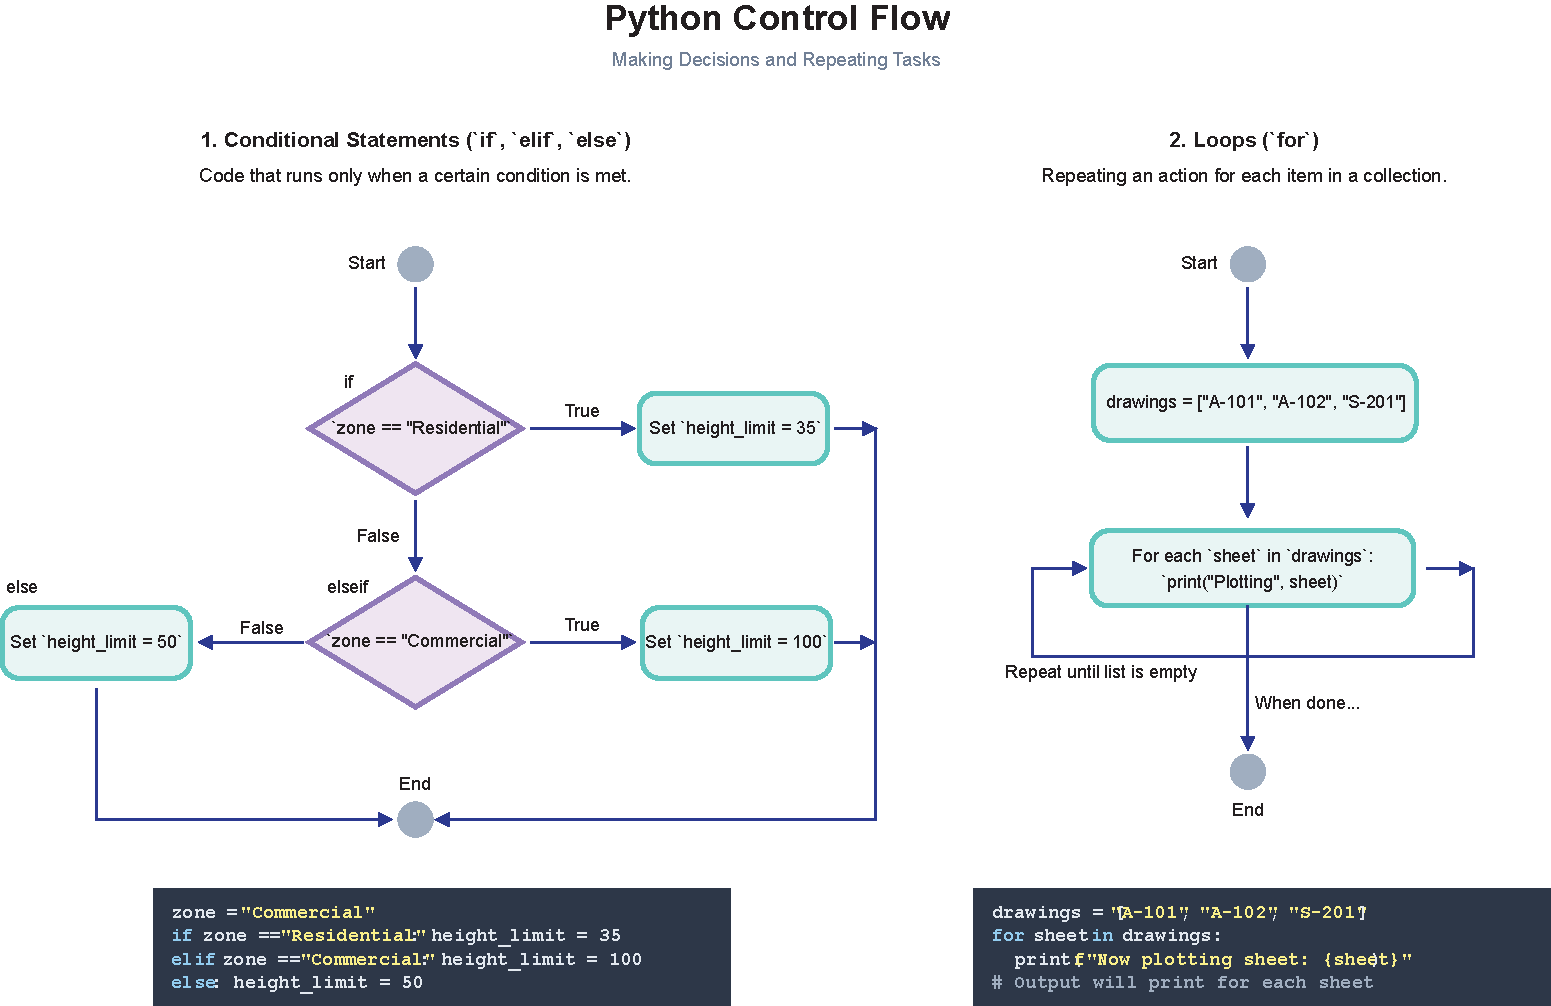
\includegraphics[width=\linewidth]{Figures/Control flow/Control_flow.pdf}
  \caption{Control flow as decisions ({if}/{elif}/{else}) and loops ({for}/{while}).}
  \label{fig:control_flow}
\end{figure}

\begin{tcolorbox}[% passing options here
    title=Focus of this chapter:,
    colframe=orange,
    colback = white,
%    colback=orange!40!yellow!30, % think of mixing 2 colors with sliders
    arc=2mm % sharp corners
 ]
    
\begin{itemize}
  \item Write \c{if}, \c{elif}, \c{else} clearly and predictably.
  \item Loop with \c{for} and control loops using \c{break}, \c{continue}, \c{pass}.
  \item Use \c{for - else} and \c{while} safely (avoid infinite loops).
  \item Recognize truthy/falsy values and use concise patterns (guard clauses, ternary).
  \item Apply these ideas to room checks, data cleanup, and budget searches.
\end{itemize}
\end{tcolorbox}

\hh{If statements}

A single decision: run a block only when a condition is True. You will use comparisons
(\c{<, <=, >, >=, ==, !=}) and logical operators (\c{and, or, not}). In Python,
\emph{indentation creates the block}.

\code{c08_if_basic}{python}{
    # 1) Define the rule and an example data point
    threshold_m2 = 9.0            # minimum acceptable area (m^2)
    room_area = 8.6               # measured area for a room

    # 2) Decision: only print when the rule is satisfied
    if room_area >= threshold_m2: # condition -> True/False
        print("OK")               # runs only when condition is True

    # Outcome: nothing prints because 8.6 < 9.0
}{Basic if: conditionally execute a block.}

\code{c08_if_equal}{python}{
    # Exact match (strings) -> case matters
    room_type = "Studio"
    if room_type == "Studio":
        print("Match: Studio")
    # Outcome:
    # Match: Studio
}{Equality check with strings (case-sensitive).}

\code{c08_if_else_basic}{python}{
    # Basic two-way choice
    area_m2 = 12.0
    min_area = 9.0
    if area_m2 >= min_area:
        print("OK")
    else:
        print("Too small")
    # Outcome:
    # OK
}{Simple if/else using a threshold.}

\code{c08_if_between}{python}{
    # Check a range with chained comparisons (reads like math)
    span_m = 7.8
    if 6.0 <= span_m <= 9.0:
        print("Span is within the 6–9 m target band")
    # Outcome:
    # Span is within the 6–9 m target band
}{Between-check with chained comparisons.}

\begin{NoteBox}
Nearly every real check—minimum widths, egress requirements,
daylight thresholds—starts with a clear \c{if}.
\end{NoteBox}

\hhh{If--else and if--elif--else chains}

Two-way and multi-way choices. Only the first True branch runs; the rest are skipped.
Order from most specific to least specific.

\code{c08_if_else_chain}{python}{
    # 1) Input score
    grade = 82

    # 2) Choose the first matching range
    if grade >= 90:
        letter = "A"              # most specific (top distinction)
    elif grade >= 80:
        letter = "B"
    elif grade >= 70:
        letter = "C"
    else:
        letter = "D"              # default (no earlier matches)

    print(letter)                 # -> B
    # Outcome:
    # B
}{Multi-way branching with if/elif/else. First True branch wins.}

\begin{NoteBox}
Place the most restrictive condition first so it wins appropriately.
Avoid overlapping ranges unless you intend them.
\end{NoteBox}

\hhh{Shorthand if--else (ternary)}

The one-line conditional expression \c{A if condition else B}. Use it for simple value
selection; do not squeeze big logic into a single line.

\code{c08_ternary}{python}{
    span_m = 7.5
    status = "OK" if span_m <= 8.0 else "Check"   # choose one of two strings
    print(status)                                  # -> OK
    # Outcome:
    # OK
}{Ternary: pick between two expressions on one line.}

\hhh{Nested if (and when to avoid it)}

An \c{if} inside another \c{if}. Acceptable for a couple of levels, but prefer flatter logic
when possible.

\code{c08_nested_if}{python}{
    # 1) A small record for a room
    room = {"name": "Studio", "area": 18.0, "type": "teaching"}

    # 2) Nested decision
    if room["type"] == "teaching":
        if room["area"] >= 16.0:
            print("Teaching room meets minimum")
        else:
            print("Teaching room undersized")
    else:
        print("Not a teaching room")
    # Outcome:
    # Teaching room meets minimum
}{Nesting shows secondary checks; keep depth small.}

\begin{NoteBox}
Deep nesting is hard to scan. Prefer guard clauses (exit early)
or combined conditions with \c{and} / \c{or} when readable.
\end{NoteBox}

\hh{Truthiness in conditions}

Empty strings/lists/dicts and zero are \emph{False}; non-empty values are \emph{True}.
This helps you write concise guards.

\code{c08_truthiness}{python}{
    # 1) Ask for optional input
    name = input("Project name (blank for none): ").strip()

    # 2) Use truthiness instead of comparing to ""
    if not name:                  # empty string is falsy -> True
        print("Unnamed project")
    else:
        print("Project:", name)
}{Use truthiness to detect empty input.}

\hh{For loops}

Iterate through items of a sequence (or any iterable): lists, tuples, strings, dicts, files.

\code{c08_for_basic}{python}{
    # Iterate over a list of floors
    levels = [1, 2, 3, 4]
    for lvl in levels:            # lvl takes each value in turn
        print("Level", lvl)
    # Outcome:
    # Level 1
    # Level 2
    # Level 3
    # Level 4
}{Iterate over a list with for.}

\code{c08_for_irregular}{python}{
    # Irregular/gapped floors: a manually curated list
    levels = [1, 2, 4, 7, 10]    # note the gaps (no 3, 5, 6, 8, 9)
    for lvl in levels:
        print("Level", lvl)
    # Outcome:
    # Level 1
    # Level 2
    # Level 4
    # Level 7
    # Level 10
}{Iterate an irregular sequence by listing exactly what you want.}

\hhh{Looping helpers: range, enumerate, zip}

Common helpers: \c{range} (indices), \c{enumerate} (index + value), and \c{zip} (pair sequences).

\code{c08_helpers}{python}{
    # range: produce 0..n-1
    for i in range(3):
        print("i:", i)            # 0, 1, 2

    # enumerate: index + item (choose start=1 to make it human-friendly)
    rooms = ["Lobby", "Cafe", "Studio"]
    for idx, name in enumerate(rooms, start=1):
        print(idx, name)          # 1 Lobby, 2 Cafe, 3 Studio

    # zip: walk two sequences side-by-side
    areas = [24.0, 35.5, 18.0]
    for name, a in zip(rooms, areas):
        print(f"{name}: {a} m^2")
    # Outcome:
    # i: 0
    # i: 1
    # i: 2
    # 1 Lobby
    # 2 Cafe
    # 3 Studio
    # Lobby: 24.0 m^2
    # Cafe: 35.5 m^2
    # Studio: 18.0 m^2
}{range, enumerate, and zip in practice.}

\code{c08_for_range}{python}{
    # Even-numbered floors only: start=2, stop=11 (exclusive), step=2
    for lvl in range(2, 11, 2):
        print("Level", lvl)
    # Outcome:
    # Level 2
    # Level 4
    # Level 6
    # Level 8
    # Level 10
}{Use range(start, stop, step) for regular patterns.}

\hh{For--else: search without flags}

The loop’s \c{else} runs only when the loop completes \emph{without} hitting \c{break}.
Perfect for search: print when found; otherwise the \c{else} reports ``not found.''

\code{c08_for_else}{python}{
    targets = [12, 15, 20, 25]
    wanted = 21

    for t in targets:
        if t == wanted:
            print("Found", t)     # success: stop early
            break
    else:
        print("Not found")        # runs only if no break happened
    # Outcome:
    # Not found
}{Use for--else instead of a manual “found” flag.}

\hh{Loop control: break, continue, pass}

\c{break} exits the loop immediately; \c{continue} skips to the next iteration;
\c{pass} does nothing—useful as a placeholder while drafting.

\code{c08_break}{python}{
    # break: stop at the first over-capacity room
    cap = 30.0
    areas = [18.0, 24.0, 31.0, 28.0]

    for a in areas:
        if a > cap:
            print("Over capacity:", a)
            break                 # leave the loop now
    # Outcome:
    # Over capacity: 31.0
}{break exits a loop right away.}

\code{c08_continue}{python}{
    # continue: skip blank lines while processing text
    lines = ["Lobby,24.0", "", "Studio,18.0", " "]
    for ln in lines:
        if not ln.strip():        # empty/whitespace-only string
            continue              # skip to next item
        print("Processing:", ln)
    # Outcome:
    # Processing: Lobby,24.0
    # Processing: Studio,18.0
}{continue jumps to the next iteration.}

\code{c08_pass}{python}{
    def TODO_validate_room(room):
        pass                      # syntactic placeholder: do nothing for now

    for a in [18.0, 20.0, 22.0]:
        if a < 0:
            pass                  # placeholder: no negative areas expected
}{pass keeps the structure valid while you draft.}

\hh{While loops (careful and useful)}

Repeat while a condition is True. Update the condition inside the loop to avoid an
infinite loop. Great for input validation, retry logic, and reading streams until a
sentinel value appears.

\code{c08_while}{python}{
    # Input guard loop: keep asking until a positive number is entered
    while True:                                  # 1) loop forever (we will break)
        txt = input("Width (m): ").strip()       # 2) read user input
        if txt and float(txt) > 0:               # 3) valid when non-empty and positive
            w = float(txt)                       #    convert once we know it's valid
            break                                # 4) leave the loop
        print("Please enter a positive number.") # feedback on invalid input

    print("Width:", w)
    # Outcome (example interaction):
    # Width (m):
    # Please enter a positive number.
    # Width (m): 5
    # Width: 5.0
}{Typical input validation with while + break.}

\hh{Guard clauses vs nested if}

Guard clauses are \emph{early exits} for invalid inputs. They reduce indentation and
make the “happy path” easy to read.

\code{c08_guard}{python}{
    def beam_capacity_ok(span_m, load_kN):
        # Guard 1: invalid inputs -> exit early
        if span_m <= 0 or load_kN <= 0:
            return False

        # Main path: compute a simple stress proxy and compare to a limit
        stress_proxy = load_kN / span_m
        return stress_proxy < 12.0
    # Outcome:
    # (Function returns True/False; try calling with example values.)
}{Use early returns to keep code flat and readable.}

\hh{Common pitfalls and fixes}

Typical mistakes to avoid immediately.

\begin{itemize}
  \item \textbf{Mis-indentation.} The block under \c{if} / \c{for} must be indented consistently.
  \item \textbf{Assignment vs equality.} \c{=} assigns; \c{==} compares. \c{if x = 3} is a syntax error.
  \item \textbf{Mutating while iterating.} Removing from a list you are looping over can skip items.
  \item \textbf{for--else misunderstanding.} \c{else} runs only if the loop did not \c{break}.
\end{itemize}

\code{c08_mutate_iter}{python}{
    # BAD: removing items while iterating the same list
    vals = [1, 2, 3, 4]
    for v in vals:
        if v % 2 == 0:
            vals.remove(v)        # modifies list in-place during iteration
    print(vals)                   # unexpected result

    # Better: build a new list with a comprehension
    vals = [1, 2, 3, 4]
    filtered = [v for v in vals if v % 2 != 0]
    print(filtered)               # [1, 3]
    # Outcome:
    # [1, 3, 4]
    # [1, 3]
}{Avoid mutating a list you are iterating.}

\hh{Worked example: budget search with for--else + break}

Use \c{for--else} to report success or “none found” without extra flags.

\code{c08_worked_search}{python}{
    rooms = [
        {"name": "Lobby", "cost": 120_000},
        {"name": "Cafe", "cost": 180_000},
        {"name": "Studio", "cost": 90_000},
    ]
    budget = 150_000

    for r in rooms:
        if r["cost"] > budget:
            print("Over budget:", r["name"], r["cost"])
            break                                   # stop at the first violation
    else:
        print("All rooms within budget")            # no break -> all were OK
    # Outcome:
    # Over budget: Cafe 180000
}{Classic search/report pattern without a separate flag.}

\hh{Mini-Lab A: Category by area}
Prompt for \c{area_m2} (float). Print \c{"small"} if \c{area_m2 < 20},
\c{"medium"} if \c{20 <= area_m2 < 40}, else \c{"large"}.

\code{c08_labA}{python}{
    area_m2 = float(input("Area (m^2): "))
    if area_m2 < 20:
        print("small")
    elif area_m2 < 40:
        print("medium")
    else:
        print("large")
}{Range-based branching.}

\hh{Mini-Lab B: Find a code with for--else}
Given \c{codes = ["RC", "GLT", "GRC", "AL"]}, ask for a target code and search with a \c{for} loop.
On match, print \c{"found"} and stop; if not found, print \c{"not found"} using the loop \c{else}.

\code{c08_labB}{python}{
    codes = ["RC", "GLT", "GRC", "AL"]
    target = input("Material code: ").strip().upper()

    for c in codes:
        if c == target:
            print("found:", c)
            break
    else:
        print("not found")
}{Search with for--else.}

\hh{Mini-Lab C: Clean lines with continue}
Given \c{lines = ["Lobby,24.0", "", "Studio,18.0", "  "]}, print only non-blank lines.
Use \c{continue} to skip blanks.

\code{c08_labC}{python}{
    lines = ["Lobby,24.0", "", "Studio,18.0", "  "]
    for ln in lines:
        if not ln.strip():
            continue
        print("Line:", ln)
}{Skip blanks using continue.}

\hh{Mini-Lab D: Retry until valid input (while + break) }
Validate and loop until the user enters a positive number for width (m).

\code{c08_labD}{python}{
    while True:
        txt = input("Width (m): ").strip()
        if txt and float(txt) > 0:
            w = float(txt)
            break
        print("Please enter a positive number.")
    print("Width:", w)
}{Input validation loop.}

\hh{Self-check}
\begin{itemize}
  \item When does the \c{else} in a \c{for} loop run?
  \item Rewrite a nested-if using a guard clause to reduce indentation.
  \item Show a case where \c{continue} is clearer than an inner \c{if/else}.
  \item Write a ternary that sets \c{label} to \c{"OK"} if \c{x <= 10} else \c{"Check"}.
  \item In your own words, why do guard clauses make code easier to read?
\end{itemize}
